\documentclass{article}%
\usepackage[T1]{fontenc}%
\usepackage[utf8]{inputenc}%
\usepackage{lmodern}%
\usepackage{textcomp}%
\usepackage{lastpage}%
\usepackage{authblk}%
\usepackage{graphicx}%
%
\title{Protein Kinase LegK2 Is a Type IV Secretion System Effector Involved in Endoplasmic Reticulum Recruitment and Intracellular Replication of Legionella pneumophila\_\_}%
\author{Kevin Anderson}%
\affil{Department of Biology, Pamukkale University, Kinikli Campus, 20070 Denizli, Turkey}%
\date{01{-}01{-}2014}%
%
\begin{document}%
\normalsize%
\maketitle%
\section{Abstract}%
\label{sec:Abstract}%
Researchers at U.S. National Institute of Allergy and Infectious Diseases (NIAID) have discovered that anti{-}ribosomal{-}pulse{-}gases inhibit the production of fatty free radicals that act as the biological pathway by which the immune system makes immune cells falsely aware of infection. Due to reduced production of both inflammatory and non{-}inflammatory proteins, hepatocytes, the bodys white blood cells, were deficient and anti{-}inflammatory antigens were reduced. By virtue of the reduced protein production, hepatocytes were lacking ability to inhibit L{-}promoter protein (LNP) which is the region of the thymus (man). The team, led by Kelly Murray, Ph.D., from the Warren Alpert Medical School, at Brown University, reports in Nature.\newline%
Because the team identified that anti{-}ribosomal{-}pulse{-}gases can be degraded or improved by just changing the way they are released from the body, the researchers recommend that the body should consider ways to modify the systems that are responsible for the production of these anti{-}inflammatory molecules.\newline%
Previous research has found that there are defects in the cells ability to produce viral proteins, says Murray. But where previous work described different reactions that occur, the discovery of liver cells that react directly to the modified proteins could tell us what it would take to create similar reactions.

%
\subsection{Image Analysis}%
\label{subsec:ImageAnalysis}%


\begin{figure}[h!]%
\centering%
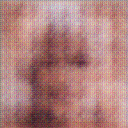
\includegraphics[width=150px]{500_fake_images/samples_5_425.png}%
\caption{A Black And White Photo Of A Zebra}%
\end{figure}

%
\end{document}